\documentclass{beamer}
\usepackage[english,french]{babel}
\usepackage[T1]{fontenc}
\usepackage[utf8]{inputenc}
\usepackage[math]{kurier}

\usepackage{graphicx, color, subfigure, wrapfig, afterpage, fancyhdr,
  graphicx, calc, url, boxedminipage, xspace, lscape, stfloats,
  todonotes, amsmath, amsthm, amssymb, mathtools, etoolbox, tikz,
  tikz-cd}

\usepackage[mathscr]{euscript}

\usetikzlibrary{shapes, calc, fadings, matrix, arrows, automata,
  positioning, decorations.markings}

\usepackage{yfonts}

\PassOptionsToPackage{hyphens}{url}\usepackage{hyperref}
\newcommand{\ok}{\scalebox{2}{\color{mycolor} \ensuremath \checkmark}}

\newenvironment{blockquote}{%
  \par%
  \medskip
  \leftskip=1.5em\rightskip=2em%
  \noindent\ignorespaces\em}{%
  \par\medskip}


\newcommand{\donc}{\ensuremath\Longrightarrow\,}
\def\Put(#1,#2)#3{\leavevmode\makebox(0,0){\put(#1,#2){#3}}}

%\everymath{\displaystyle}

\definecolor{mycolor}{HTML}{484BBA}
\definecolor{mycolor2}{HTML}{73A0C5}

\definecolor{MYblue}{HTML}{73A0C5}
\definecolor{MYlightbrown}{HTML}{D2965A}
\definecolor{MYdarkblue}{HTML}{072e39}
\definecolor{MYdarkbrown}{HTML}{86592C}
\definecolor{MYlightblue}{HTML}{2C7186}
\definecolor{MYgreen}{HTML}{5AA866}
\definecolor{MYred}{HTML}{FF4748}

\definecolor{AA}{HTML}{572762}
\definecolor{A}{HTML}{1A5882}
\definecolor{B}{HTML}{713657}
\definecolor{C}{HTML}{0C8F7F}
\definecolor{D}{HTML}{914747}
\definecolor{E}{HTML}{446E8F}
\definecolor{F}{HTML}{10633D}

\usetheme{Goettingen}
\usecolortheme{spruce}

\setbeamercolor{section in sidebar shaded}{fg=gray}
\setbeamercolor{palette sidebar secondary}{fg=black}

\setbeamertemplate{navigation symbols}{} 
\setbeamertemplate{footline}{
  \hfill 
%  {\em \scriptsize  \insertsection} 
  \hspace*{1em}
  \footnotesize  \it \insertframenumber 
  \hspace*{1em} \vspace*{1em}
}


%% \setbeamertemplate{blocks}[default, shadow=true]
%% \useinnertheme{rectangles}


 \newcommand{\transition}[1]{
   \mode<all> {
     \setbeamercolor{background canvas}{bg=structure.fg}
   }

   \begin{frame}<handout:0>[plain,noframenumbering]
     \centering
     \color{white}
     \vspace{4em}
    
     {\Huge #1}
     \vfill
    
   \end{frame}
   \mode<all> {
     \setbeamercolor{background canvas}{bg=white}
   }
 }


%--------------------------------------------------------------------------
% General presentation settings
%--------------------------------------------------------------------------
\title{Apprentissage par renforcement}
\date{October 2016}

\author{Sergey Kirgizov}

\institute[UB]{Université de Bourgogne}

\begin{document}

\maketitle

\section{Intro}

\begin{frame}[t]{Exemple motivant}{Jeu du loup}

  \begin{center}
    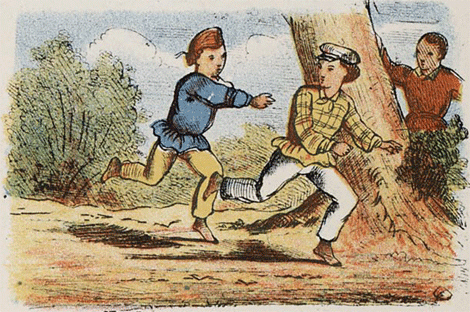
\includegraphics[width=12em]{figs/Jongensspelen_10.jpg}
  \end{center}


  \hspace*{4em}\only<2-4>{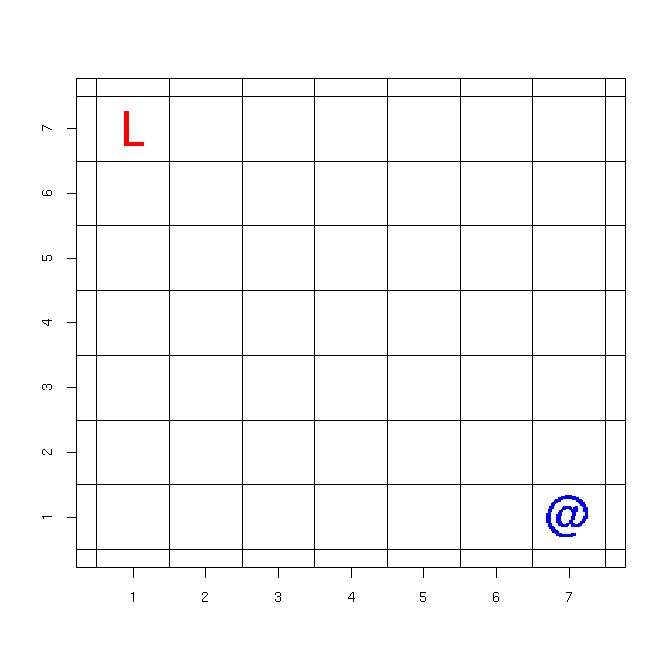
\includegraphics[width=8em]{figs/bad.png}}\quad\only<4>{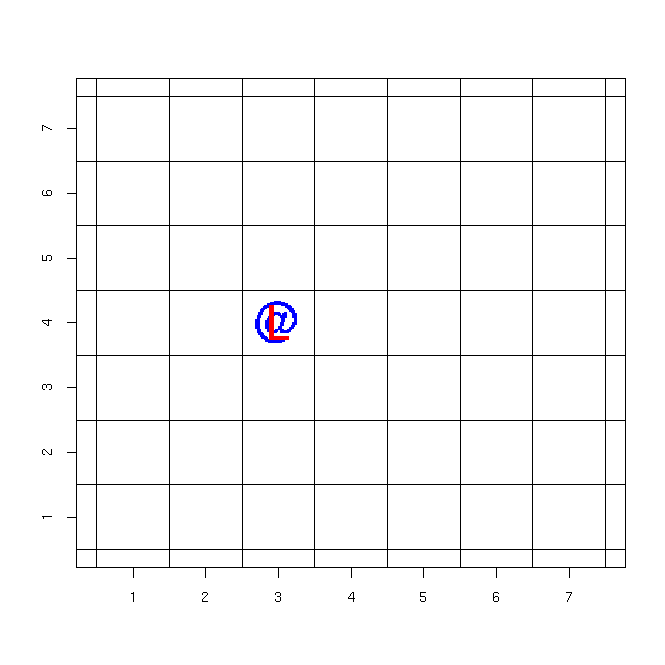
\includegraphics[width=8em]{figs/good.png}}

  \vspace*{-1em}
  \only<2-4>{\hspace*{0em} Pas bien pour le loup  $\uparrow$}
  \only<3,4>{
    \Put(-80,155){\scalebox{0.5}{
        \begin{tabular}{ccc}
          $\nwarrow$&$\uparrow$&$\nearrow$\\
          $\leftarrow$&$\cdot$&$\rightarrow$\\
          $\swarrow$&$\downarrow$&$\searrow$
        \end{tabular}
      }}
    \Put(-27.5,53.5){\scalebox{0.5}{
        \begin{tabular}{ccc}
          $\nwarrow$&$\uparrow$&$\nearrow$\\
          $\leftarrow$&$\cdot$&$\rightarrow$\\
          $\swarrow$&$\downarrow$&$\searrow$
        \end{tabular}
      }}
  }
  \vspace*{-1.5em}
  \only<4>{\hspace*{15em} $\uparrow$ Bien pour le loup}
\end{frame}


\begin{frame}{Idée l'apprentissage par renforcement}

\end{frame}

\section{Historique}

\begin{frame}{Historique}
  \begin{itemize}
  \item[1988] TD-learning, Richard Sutton\hspace{1em}
    \raisebox{-.5\height}{%
      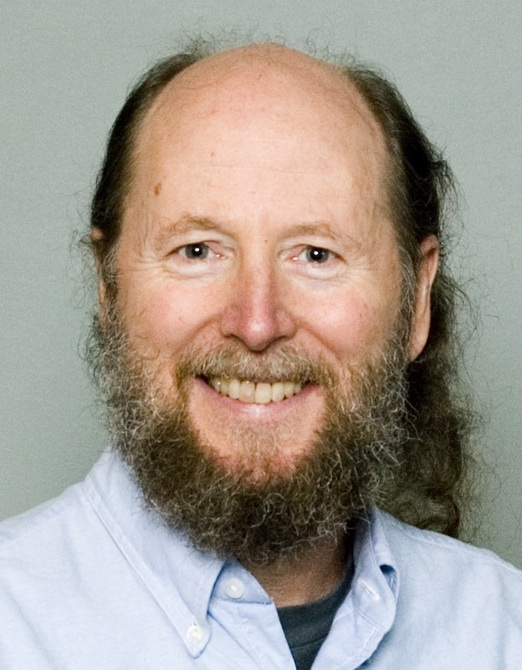
\includegraphics[width=6em]{figs/Sutton-head5.jpg}}
    
  \item[1989] Q-learning,  Chris Watkins\hspace{1.8em}
    \raisebox{-.5\height}{
      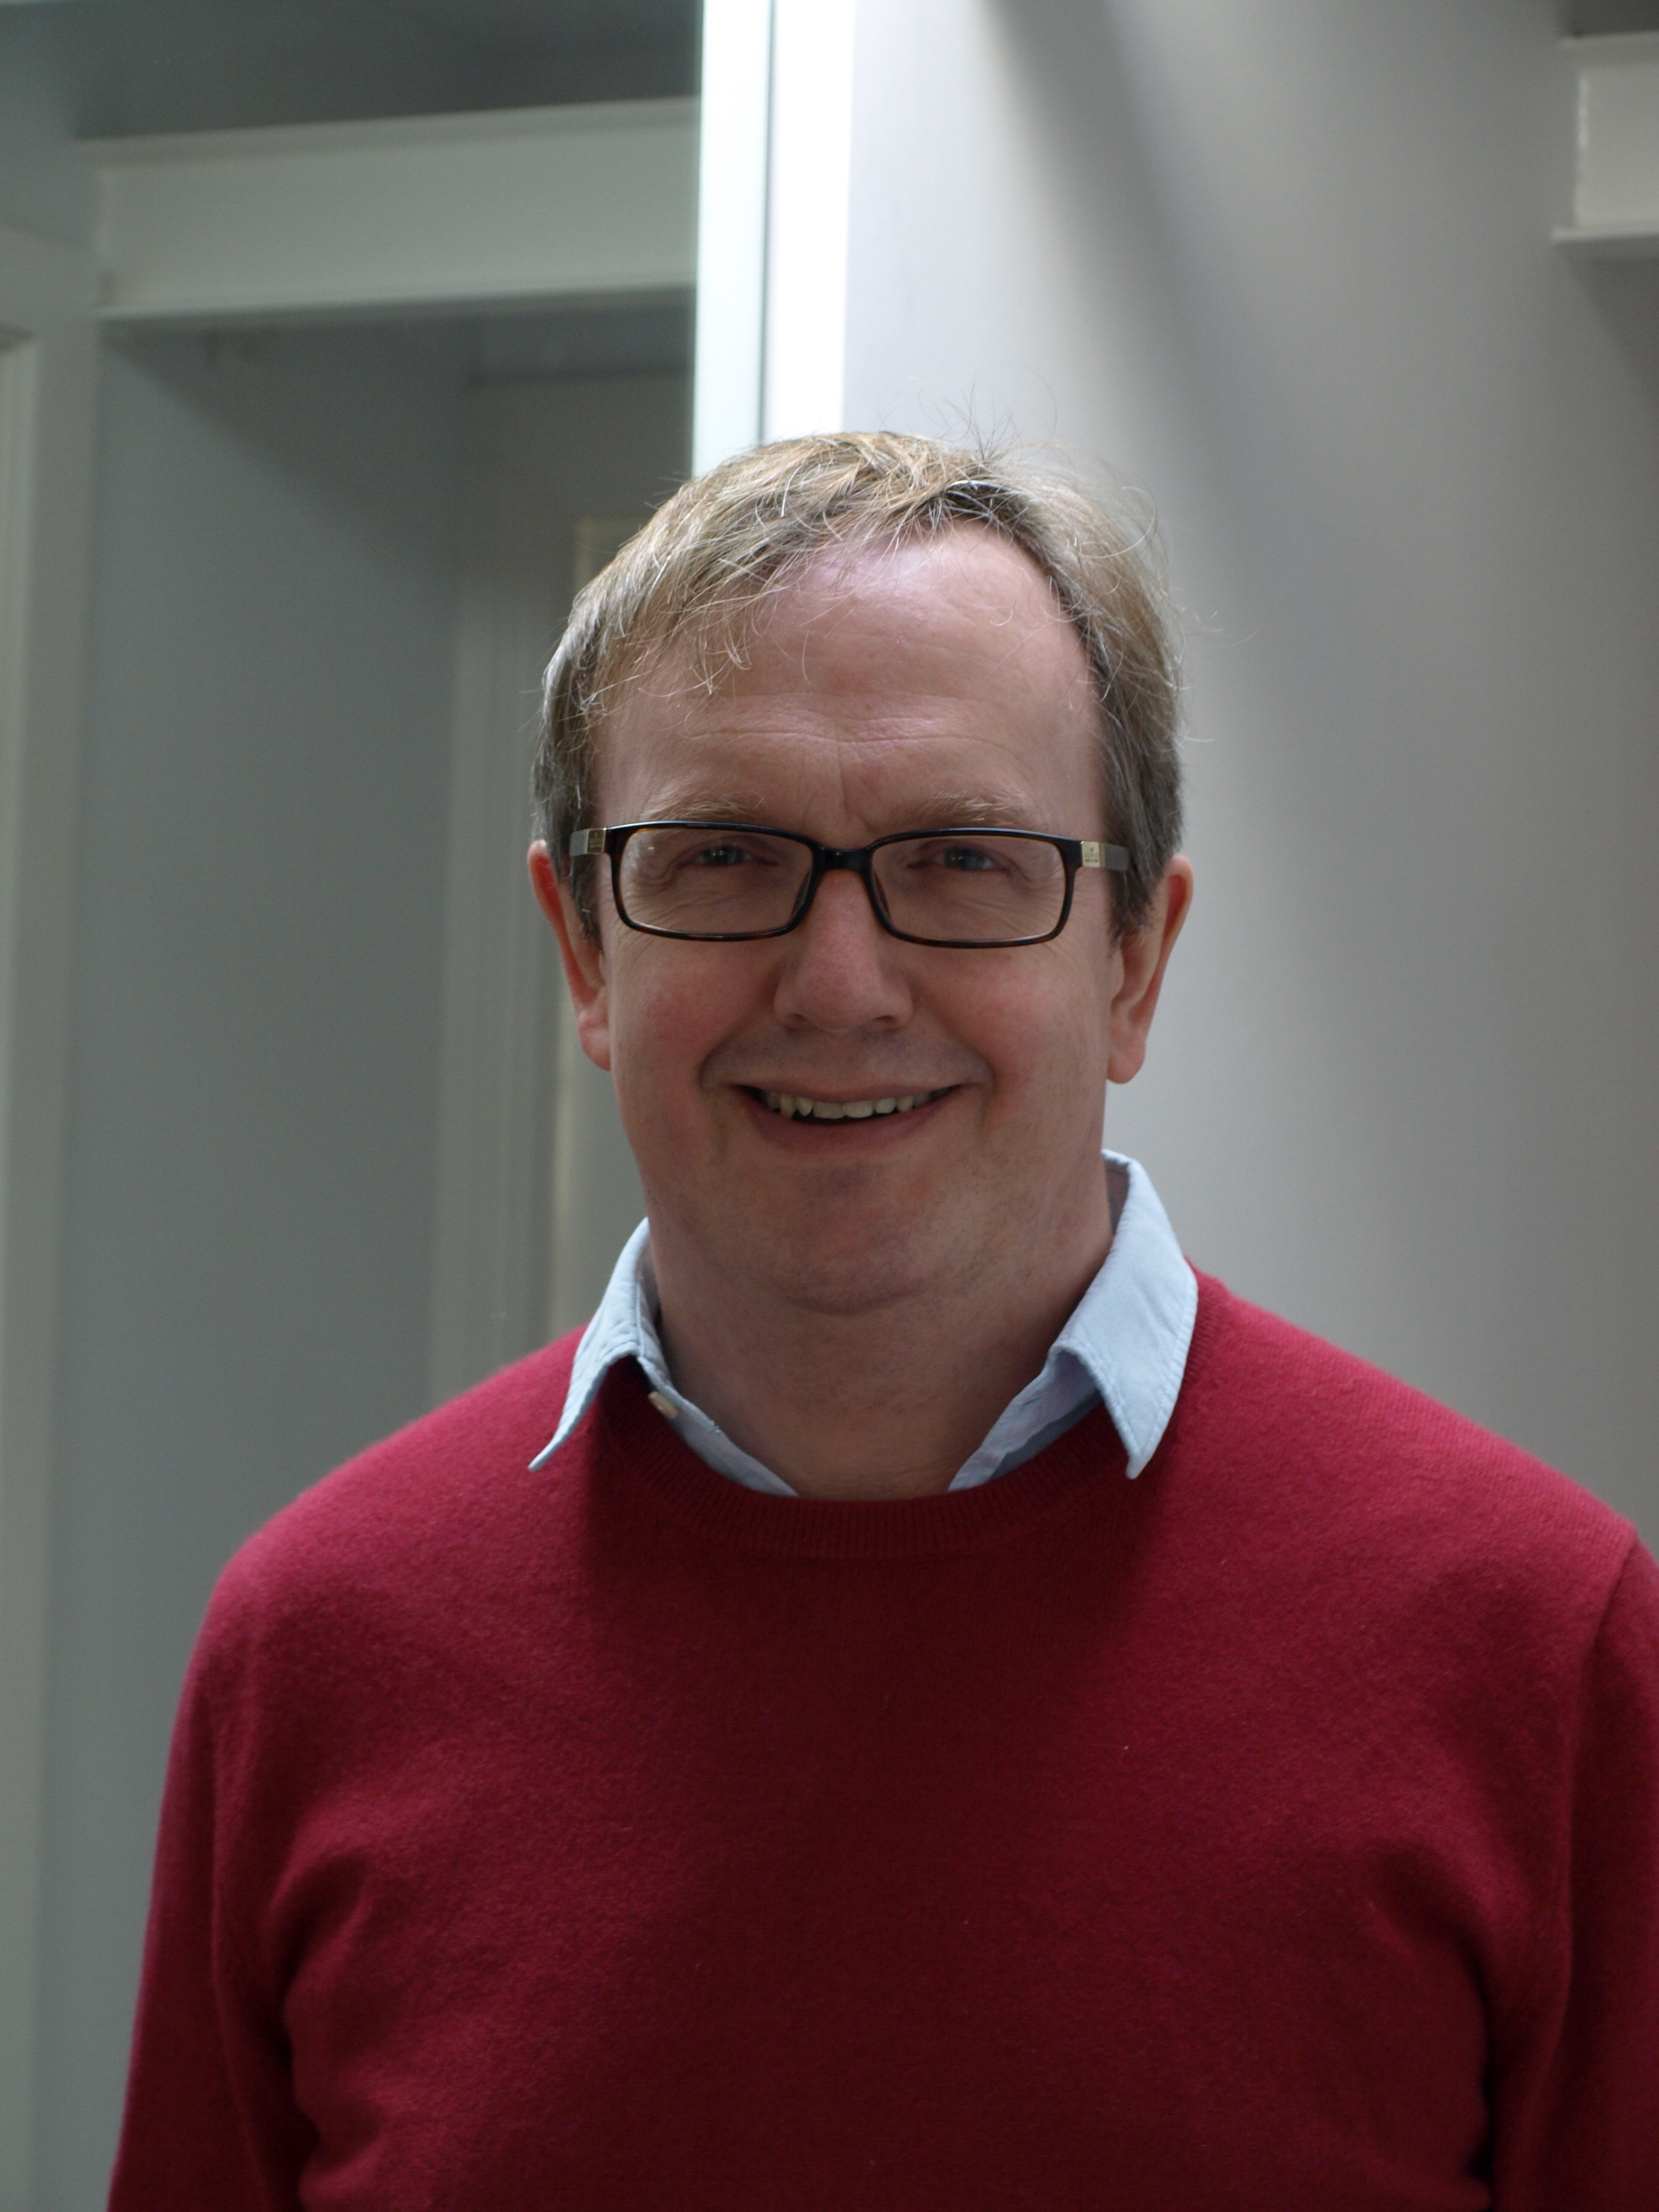
\includegraphics[width=6em]{figs/cw090311.jpg}}
    
  \end{itemize}
\end{frame}
  
\begin{frame}{Historique}

``Toutefois, l'origine de l'apprentissage par renforcement est plus
ancienne. Elle dérive de formalisations théoriques de méthodes de
contrôle optimal, visant à mettre au point un contrôleur permettant de
minimiser au cours du temps une mesure donnée du comportement d'un
système dynamique. La version discrète et stochastique de ce problème
est appelée un processus de décision markovien et fut introduite par
Richard Ernest Bellman en 1957''

\centering
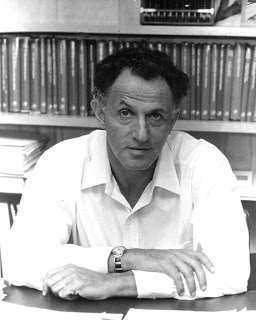
\includegraphics[width=6em]{figs/Bellman.jpg}

\hfill \scriptsize \url{https://fr.wikipedia.org/wiki/Apprentissage_par_renforcement}

\end{frame}


\begin{frame}{Théories de psychologie animale $\to$ Intelligence artificielle }
  ``D'autre part, la formalisation des problèmes d'apprentissage par
  renforcement s'est aussi beaucoup inspirée de théories de
  psychologie animale, comme celles analysant comment un animal peut
  apprendre par essais-erreurs à s'adapter à son environnement. Ces
  théories ont beaucoup inspiré le champ scientifique de
  l'intelligence artificielle et ont beaucoup contribué à l'émergence
  d'algorithmes d'apprentissage par renforcement au début des années
  1980.''

  \hfill \scriptsize --- Wikipedia
\end{frame}


\begin{frame}{Livres}

\begin{enumerate}
\item {\bf Reinforcement Learning: An Introduction}

Richard S. Sutton et Andrew G. Barto

\item {\bf Processus décisionnels de Markov en intelligence artificielle}

Olivier Sigaud et  Olivier Buffet
\end{enumerate}


\begin{center}
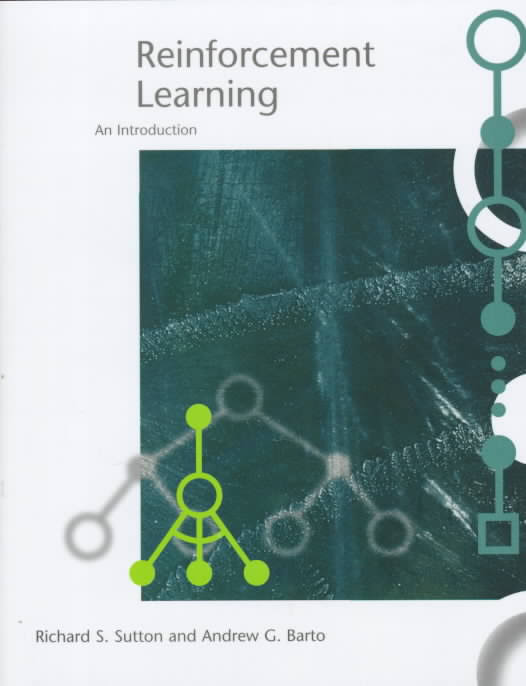
\includegraphics[width=8em]{figs/rl-book.jpeg}
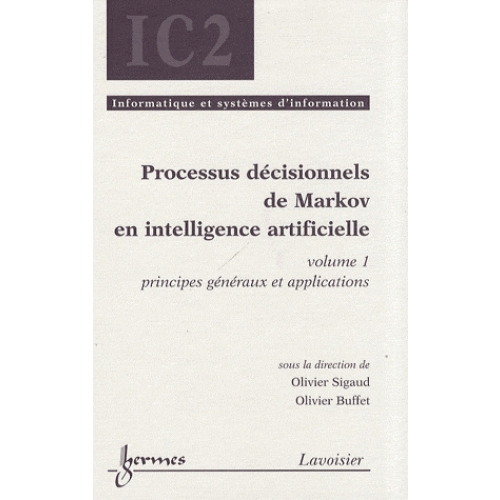
\includegraphics[width=12em]{figs/book21.jpg}
\end{center}
\end{frame}


\begin{frame}{draft}
  Markov Decision Process (MDP)
  
  Finite and small are easy. (better than bruteforce???)
  
  But large and (infinity) are difficult.
  How to explore?
  
  ballance between explorations and actions
  
  Q-learning is an exemple of a stochastic approximation algorithm
\end{frame}


\section{Théorie}

\begin{frame}{Definitions}
  $S$ est un ensemble d'états

  $A$ est un ensemble d'actions

  $\Pi : S \to A$ est une politique

  rules of transitioning between states;
  
  rules that determine the scalar immediate reward of a transition;

  and rules that describe what the agent observes.
  
  TODO: cite some books
\end{frame}

\begin{frame}

{\bf !!! Q-Learning is an Off-Policy algorithm for Temporal Difference learning!!!}

Types of Reinforcement Learning:
\begin{enumerate}
\item Bruteforce
\item TD-learning
\item Q-learning
\item Bellman equation ?
\item other stuff
\end{enumerate}
\end{frame}


\section{Q-learning}

\begin{frame}{Q-learning}
    
  \begin{multline*}
    Q_{t+1}(s_t,a_t) = Q_t(s_t,a_t) (1 - \alpha) + \\
                     \alpha \left( r_{t+1} + \gamma \max_a Q_t(s_{t+1},a)     \right)
  \end{multline*}

\end{frame}


\begin{frame}{Action selection}
\end{frame}

\begin{frame}{Optimal policy...}
\end{frame}

\begin{frame}{Convergence}


Stochastic approximation algorithms by Robbins-Monro,
or Kiefer-Wolfowitz, Blume from 1950-th..



$\sum_{n=0}^\infty$ from 1950-th...
\end{frame}



\section{Applications}

% Thus, reinforcement learning is particularly well suited to problems
% which include a long-term versus short-term reward trade-off. It has
% been applied successfully to various problems, including robot
% control, elevator scheduling, telecommunications, backgammon,
% checkers (Sutton \& Barto 1998, Chapter 11) and go (AlphaGo).


\begin{frame}{AlphaGo}
  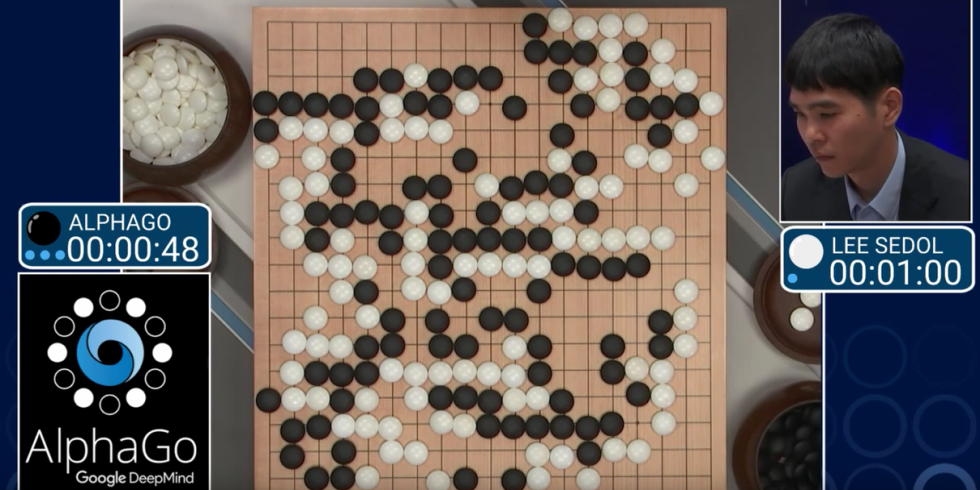
\includegraphics[width=\textwidth]{figs/alphago.png}

  \vspace{1ex}

  ``This program was based on general-purpose AI methods {\bf
    [including reinforcement learning]}, using deep neural networks to
  mimic expert players, and further improving the program by learning
  from games played against itself.''

  \hfill \scriptsize --- \url{https://deepmind.com/research/alphago}
\end{frame}


\begin{frame}{Allocation des ressources dans le cloud}
  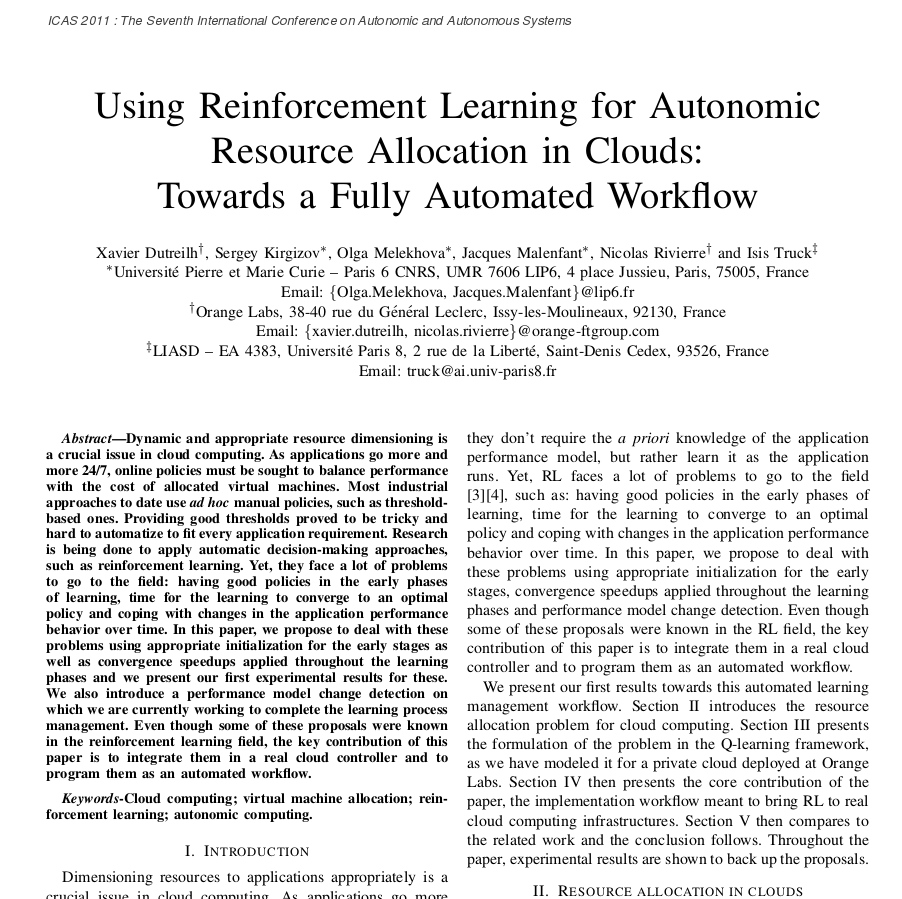
\includegraphics[width=\textwidth]{figs/mypaper.png}
\end{frame}


\begin{frame}{Neurobiologie}

  \begin{center}
    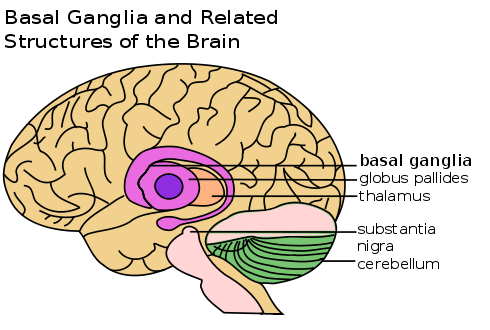
\includegraphics[width=12em]{figs/ganglions-de-base.png}
  \end{center}

  ``La collaboration entre neurobiologistes et chercheurs en
  intelligence artificielle a permis de découvrir qu'une partie du
  cerveau fonctionnait de façon très similaire aux algorithmes
  d'apprentissage par renforcement.'' 

  \hfill \scriptsize --- Wikipedia

  \vspace{1em}

  {\bf A Model of How the Basal Ganglia Generate and Use Neural Signals that Predict Reinforcement}  \\
  \hfill James C. Houk,  J. L. Adams, A. G. Barto



\end{frame}

% Le raffinement actuel des algorithmes d'apprentissage par
% renforcement inspire les travaux des neurobiologistes et des
% psychologues pour la compréhension du fonctionnement du cerveau et
% du comportement animal.

% tels que le TD-learning. Il semblerait ainsi que la nature ait
% découvert, au fil de l'évolution, une façon semblable à celles
% trouvées par des chercheurs pour optimiser la façon dont un agent ou
% organisme peut apprendre par essais-erreurs. Ou plutôt, les chercheurs
% en intelligence artificielle ont redécouvert en partie ce que la
% nature avait mis des millions d'années à mettre en place.

\section{Jeu du loup en R}

\begin{frame}[t]{Jeu du loup}{en R}
  \begin{center}
    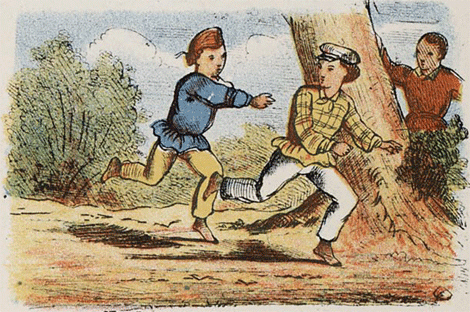
\includegraphics[width=6em]{figs/Jongensspelen_10.jpg}
  \end{center}

  Code source: \url{https://github.com/kerzol/jeu-du-loup}

  \vspace{2em}

  \hspace*{4em}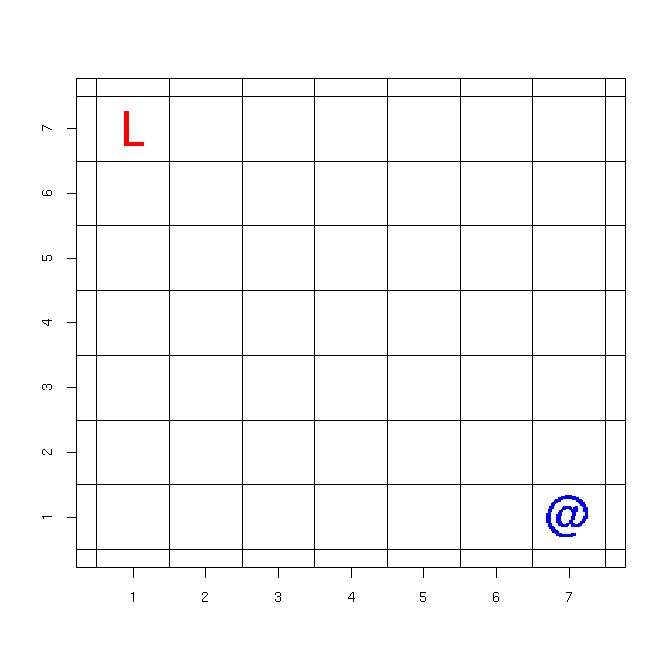
\includegraphics[width=8em]{figs/bad.png}\quad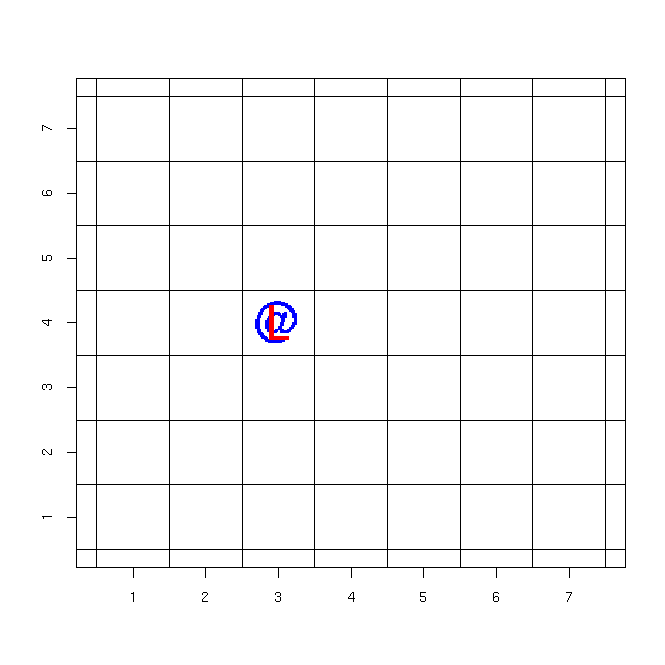
\includegraphics[width=8em]{figs/good.png}

  \vspace*{-1em}
  \hspace*{0em} Pas bien pour le loup  $\uparrow$ 
  \Put(-76.5,156){\scalebox{0.5}{
      \begin{tabular}{ccc}
        $\nwarrow$&$\uparrow$&$\nearrow$\\
        $\leftarrow$&$\cdot$&$\rightarrow$\\
        $\swarrow$&$\downarrow$&$\searrow$
      \end{tabular}
    }}
  \Put(-23.5,53.5){\scalebox{0.5}{
      \begin{tabular}{ccc}
        $\nwarrow$&$\uparrow$&$\nearrow$\\
        $\leftarrow$&$\cdot$&$\rightarrow$\\
        $\swarrow$&$\downarrow$&$\searrow$
      \end{tabular}
    }}
  
  \vspace*{-1.5em}
  \hspace*{15em} $\uparrow$ Bien pour le loup



\end{frame}




\section{En TP / Home work}

\begin{frame}{En TP / Home work}

  \begin{enumerate}
  \item Télécharger le code source : \url{https://github.com/kerzol/jeu-du-loup}
  \item Jouer avec le code
  \item Trouvez et décrire les différences entre {\tt q-loup.R} et {\tt q-loup-1.R}
  \item Pourquoi {\tt q-loup-1.R} apprend mieux le comportement cyclique du chat ?
  \item Visualisez l'evolution de valeurs de $Q$
  \item Change {\tt ALPHA = 0.6} dans le code par quelque chose qui
    respecte la condition $\sum_{i=0}^\infty \alpha_i < \infty$
  \item Ajouter quelques murs dans l'environnement.
  \end{enumerate}
\end{frame}


\section{Recherche actuelle}

\begin{frame}{Recherche actuelle et future}

\begin{itemize}
\item Environnements sont plus grands
\item Il faut augmenter la vitesse de convergence
\item Combinaison avec d'autres techniques d'apprentissage par machine
  (les réseaux de neurones, etc)
\end{itemize}
\end{frame}



\end{document}

